\input{text/diss}

\begin{document}

\def\labauthors{Войтович Д.А., Карусевич А.А., Разова А.А.}
\def\labgroup{440}
\def\labnumber{1}
\def\labtheme{Исследование твердотельных структур методом ЭПР-спектроскопии}
\renewcommand{\vec}{\mathbf}
\renewcommand{\Re}{\operatorname{Re}}
\renewcommand{\Im}{\operatorname{Im}}
\renewcommand{\phi}{\varphi}
\renewcommand{\hat}{\widehat}

\input{text/titlepage}

\section{Вступление}
\subsection*{Идея}
Метод электронного парамагнитного резонанса (ЭПР) является одним из основных методов исследование физических свойств вещества. Цель данной работы - ознакомление с теорией парамагнетизма, методом ЭПР-спектроскопии и его возможностями при исследовании твердотельных парамагнитных веществ. 

Парамагнитный резонанс представляет собой явление резонансного поглощения энергии электромагнитного поля системой парамагнитных частиц, помещенных в постоянное магнитное поле и взаимодействующих при этом с переменным высокочастотным магнитным полем. Парамагнитными называют такие вещества, элементарные частицы которых имеют суммарный магнитный момент, отличный от нуля. При этом магнитные свойства частиц обусловлены наличием нескомпенсированного спинового момента. В случае, когда магнитные моменты частиц обусловлены неспаренными электронами внешней оболочки, говорят об электронном парамагнитном резонансе. Более широкое понятие парамагнитного резонанса в макроскопических системах включает всю совокупность явлений, наблюдаемых при квантовых переходах между энергетическими уровнями системы под влиянием переменного магнитного поля резонансной частоты. 

Электронный парамагнитный резонанс наблюдается в веществах, имеющих неспаренные электроны. В то же время заполненные электронные оболочки не приводят к появлению у атома или иона парамагнитных свойств, так как в этом случае спиновый и орбитальный моменты количества движения равны нулю, и магнитный момент отсутствует. Квантовые переходы, наблюдаемые при ЭПР, лежат, как правило, в области СВЧ-диапазона. Поскольку вероятность спонтанных переходов в дипольном приближении пропорциональна третей степени частоты, в отличие от магнито-дипольных переходов оптического диапазона в методе ЭПР необходимым элементом является присутствие внешнего высокочастотного поля. Это переменное поле при условии резонанса частоты вызывает вынужденное поглощение электромагнитной энергии, регистрация которого позволяет фиксировать данное явление. В целом явление ЭПР может наблюдаться у широкого класса веществ, частицы которых обладают нескомпенсированным электронным спином. В данной работе в качестве объектов исследования взаимодействия парамагнитного вещества с внешним магнитным полем предлагаются свободный радикал дефенил-пикрил-гидразила и парамагнитный кристалл рубина с активными ионами $Cr^{3+}$.

\subsection{Установка}
Экспериментальная установка по наблюдению сигнала поглощения ЭПР собрана по схеме СВЧ-спектроскопии. Блок-схема радиоспектрометра ЭПР, используемого в данной работе, представленна на рис.1:
\begin{figure}[h!]
	\centering
	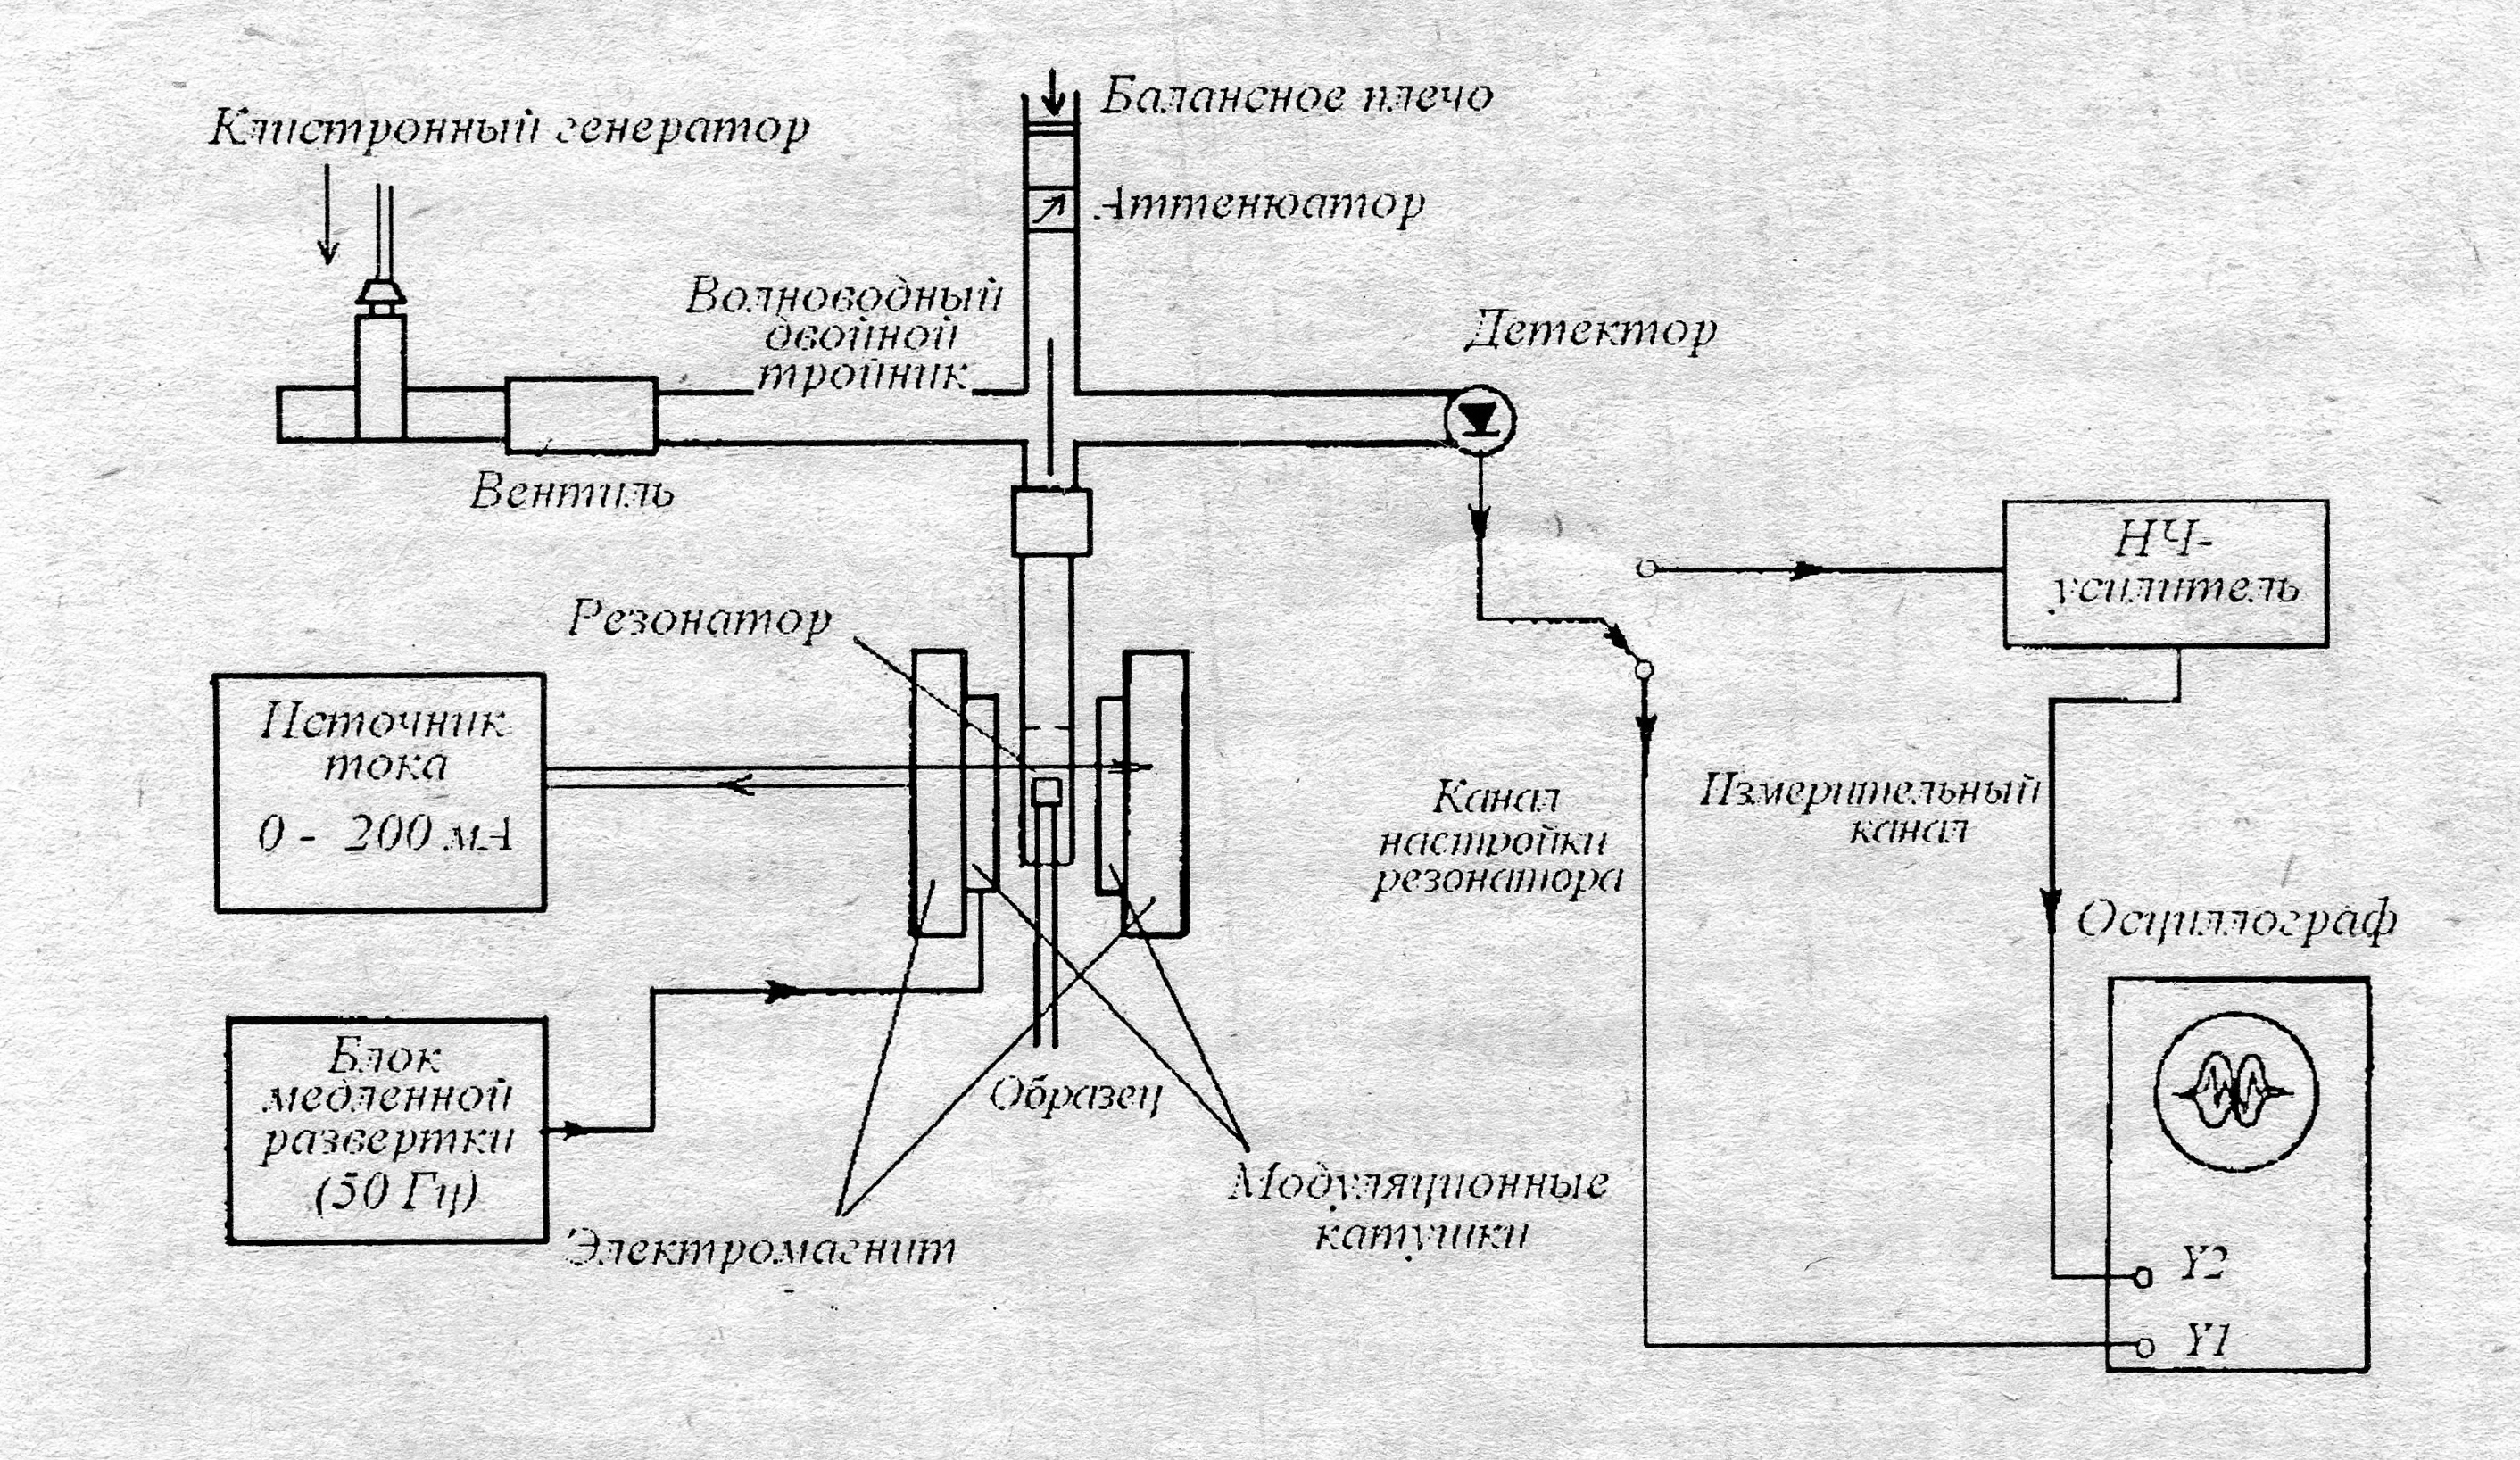
\includegraphics[width=\linewidth]{fig/Sh.jpg}
	\caption{Блок-схема ЭПР-спектрометра}
	\label{fig:1}
\end{figure}

Рассмотрим кратко работу ЭПР-спектрометра. Сигнал с клистронного генератора, который является источником излучения высокочастотного поля $\vec{H_1}(\lambda \approx$ 3 см), через ферритовый вентиль поступает во входное плечо двойного тройника. двойной тройник, собранный по мостовой схеме, служит для разделения мощности на две равные части. Одна часть поступает в балансное плечо, а другая - в резонатор. В выходное плечо волновода, подключенное к детекторной камере, сигнал от СВЧ-генератора напрямую не поступает. Отражательный резонатор представляет собой отрезок прямоугольного волновода, в котором возбуждаются колебания. В торцевых стенках резонатора имеются отверстия. Одно из них предназначено для связи резонатора с волноводом, другое - для ввода образца в резонатор. Резонатор с исследуемым образцом располагается между полюсами электромагнита, причем таким образом, что возбуждаемое в резонаторе внешним СВЧ-генератором поле $\vec{H_1}$ оказывается перпендикулярным внешнему полю $\vec{H_0}$ электромагнита. В результате взаимодействия магнитного поля с парамагнитным веществом возникает сигнал, который поступает в выходное плечо двойного тройника и детектируется, Уровень мощности сигнала можно контролировать, например, с помощью осциллографа или миллиамперметра, подключенного к детекторной камере. Продетектированный сигнал поступает на регистрирующую часть установки, состоящую из высокочувствительного усилителя переменного напряжения и осциллографа. 

Для наблюдения сигналов ЭПР на осциллографе предусмотрена низкочастотная модуляция постоянного магнитного поля $\vec{H_0}$. Эта дополнительная медленная модуляция осуществляется с помощью специальных моделирующих катушек, запитываемых от сетевого напряжения через трансформатор. Уровень постоянного магнитного поля может изменяться в пределах от 0 до 4500 эрстед с помощью системы питания катушек электромагнита на основе источника постоянного тока. На рис.2 приведена схема, поясняющая условие появления сигнала ЭПР на экране осциллографа.
\begin{figure}[h!]
	\centering
	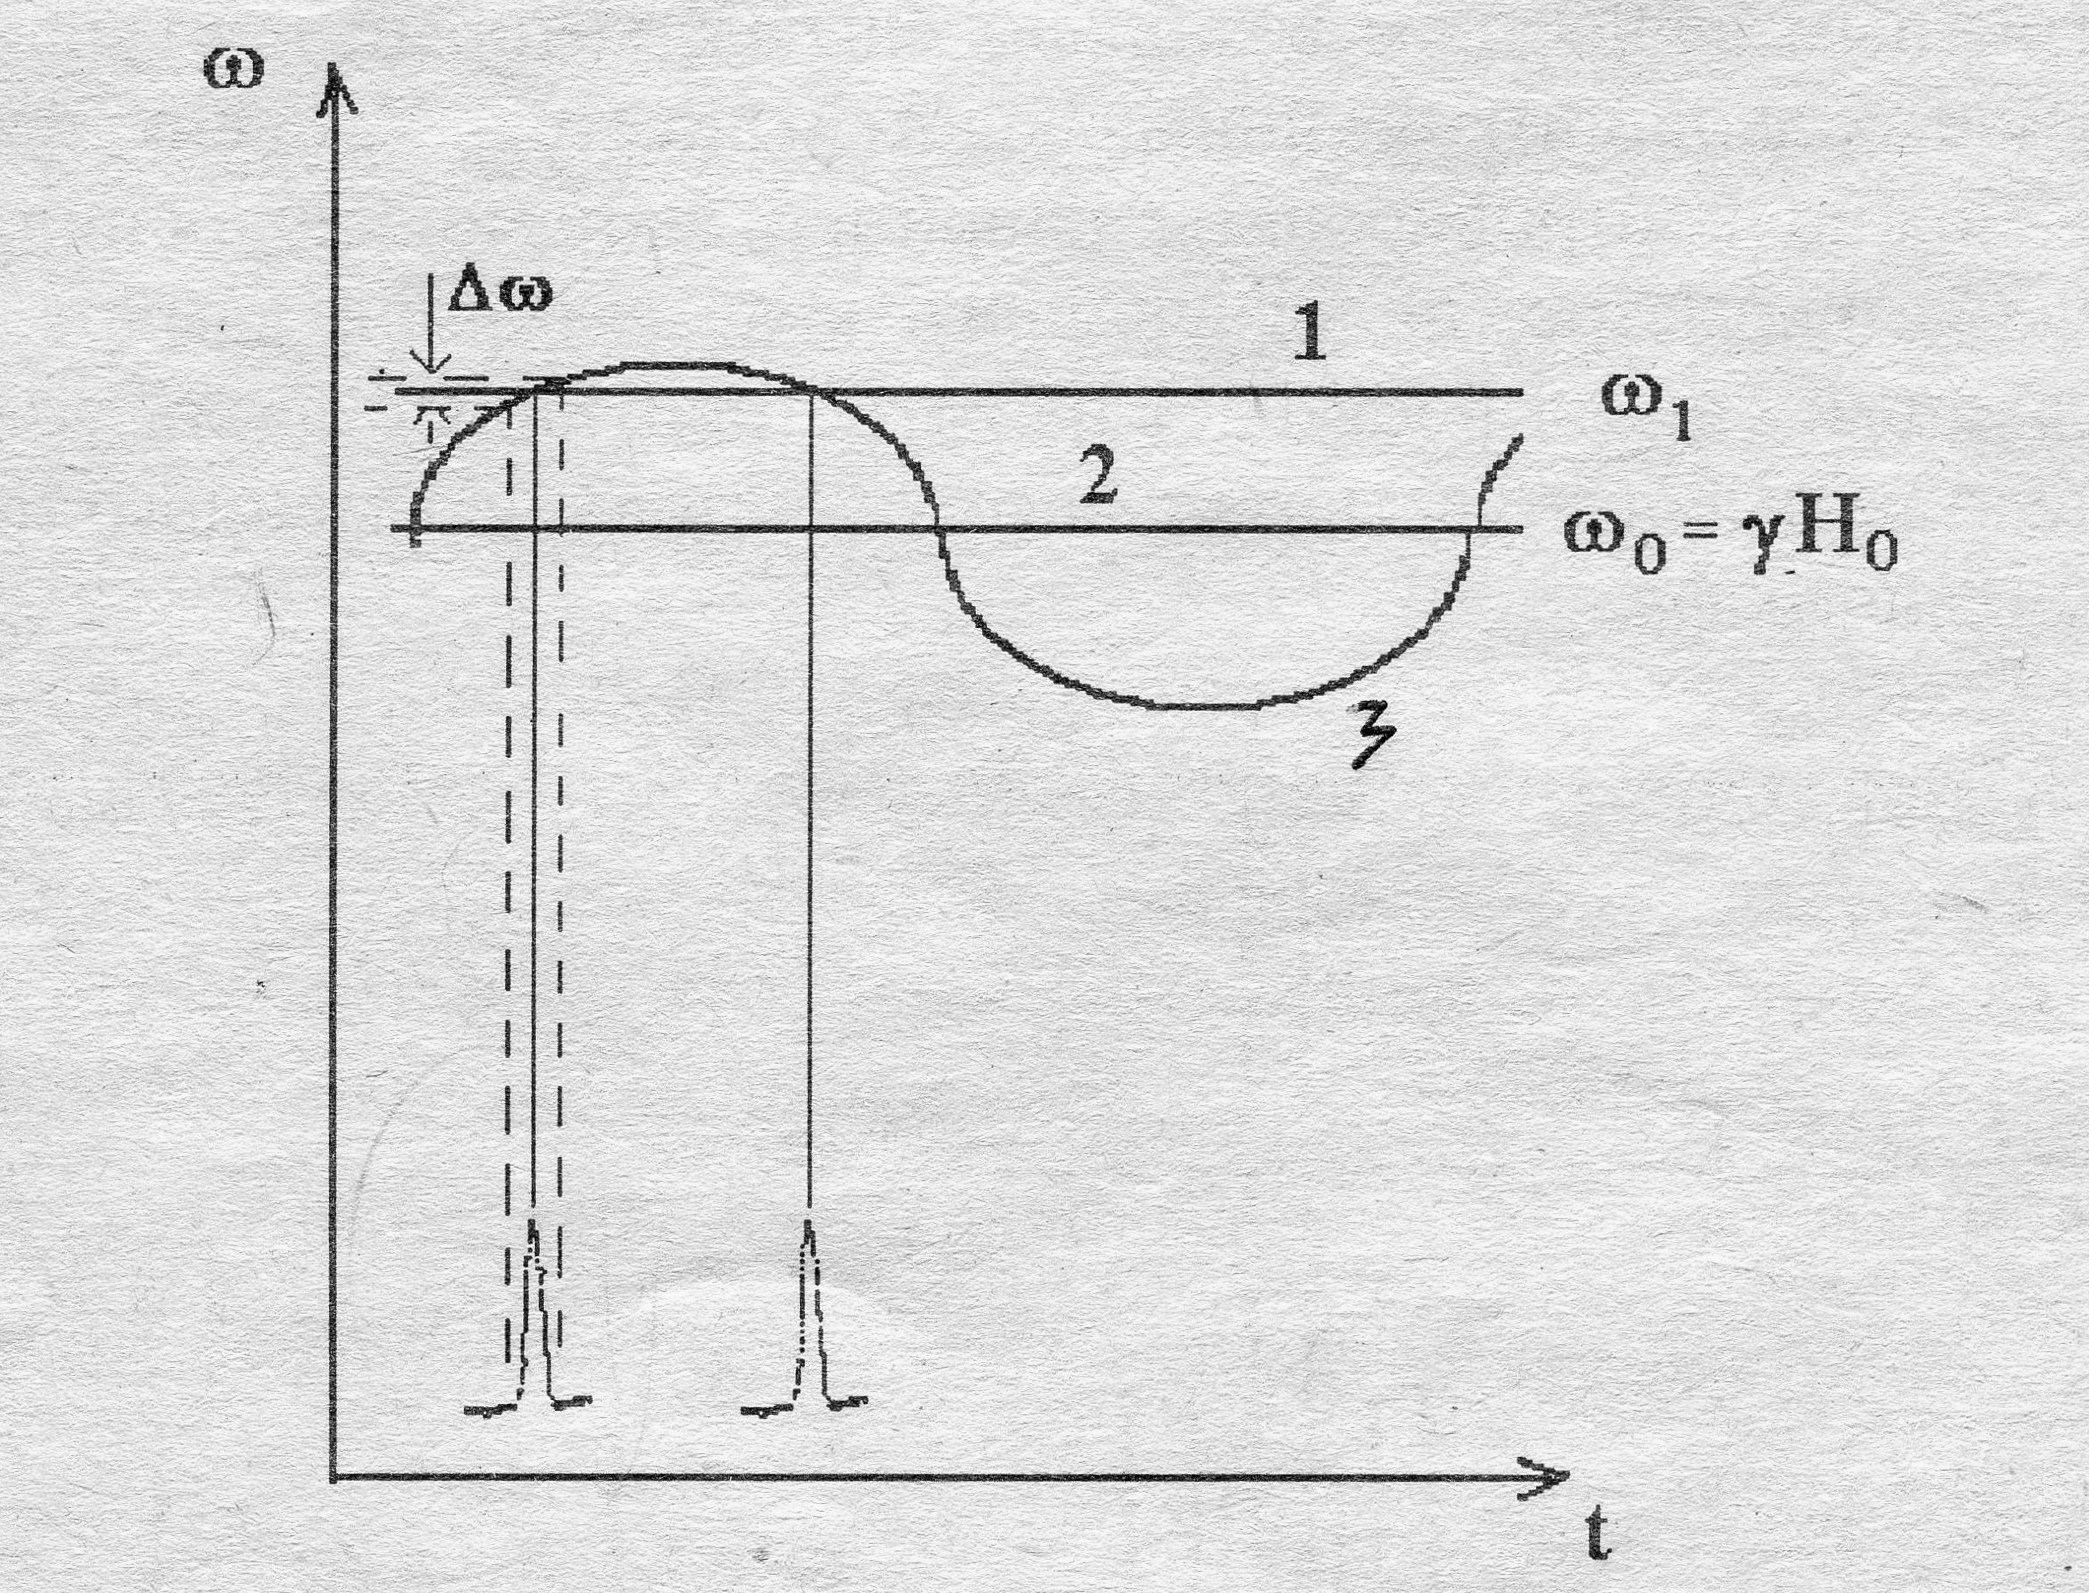
\includegraphics[width=0.7\linewidth]{fig/om(t).jpg}
	\caption{Модуляционная методика выделения сигналов ЭПР}
	\label{fig:1}
\end{figure}

 На этом графике по горизонтальной оси показано время (синхронизированное с разверткой осциллографа), по вертикальной оси - СВЧ-частота (или - с точностью до коэффициента - мгновенное значение магнитного поля в катушках). 

 Линия 1 обозначает частоту клистронного генератора, линия 2 - частоту прецессии $\omega_0$ парамагнитных частиц в веществе под воздействием внешнего постоянного поля $\vec{H_0}$. как видно из графика, наличие синусоидальной модуляции приводит к стому, что за один период развертки дважды наступает условие резонанса. Поэтому на экране осциллографа при попадании в зону резонанса одновременно наблюдается два сигнала ЭПР. 

Вследствие дисперсии магнитной восприимчивости парамагнитного образца в условиях ЭПР кроме поглощения энергии СВЧ-поля изменяется и собственная частота резонатора. Это приводит к тому, что форма наблюдаемого сигнала ЭПР определяется не только поглощением, т.е. кривой $\chi''$, но и содержит примесь дисперсионной зависимости $\chi'$, имеющей вид производной от сигнала поглощения. Для исключения возможного влияния дисперсии на форму сигнала ЭПР служит балансное плечо. Эта часть волноводной системы представляет собой переменную нагрузку и состоит из аттенюатора и замыкающего поршня, с помощью которых можно менять амплитуду и фазу отраженного в этом плече сигнала. При наличии балансного плеча на детектор одновременно поступают сигналы, отраженные от переменной нагрузки и резонатора. В зависимости от соотношения фаз этих сигналов выделенная на детекторе составляющая сигнала может быть пропорциональна или кривой поглощения, или кривой дисперсии. 

\section{Эксперимент}
\subsection{ЭПР в молекулах дифенила}
Измерения проводятся с использованием образца дифенила (дефинилпикрилгидразила). Для наблюдения кривых поглощения и дисперсии необходимо вывести на резонанс значение поля $H_0$. Определяется оно по появлению на экране осциллографа пары сигналов, соответствующих резонансному переходу. Перемещая плунжер балансного плеча можно получить следующие кривые:
\begin{center}
\begin{minipage}{0.45\linewidth}
        \centering
        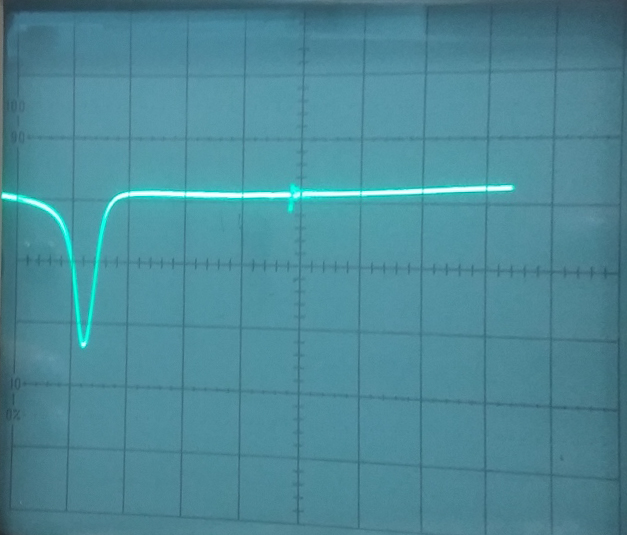
\includegraphics[width=\linewidth]{fig/chi_p-2.jpg}  
        \vspace{-20pt}
        \label{fig:4}
        \captionof{figure}{Кривая поглощения} 
    \end{minipage} 
\hfill     
    \begin{minipage}{0.45\linewidth}
        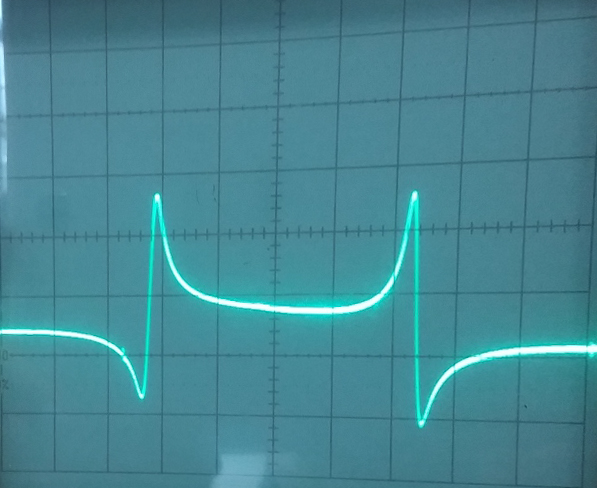
\includegraphics[width=\linewidth]{fig/chi_d-2.jpg} 
        \vspace{-20pt}
        \label{fig:3}
        \captionof{figure}{Дисперсионная кривая} 
      \end{minipage}
\end{center} 

Теоретический вид этих же кривых:
\begin{figure}[H]
	\centering
	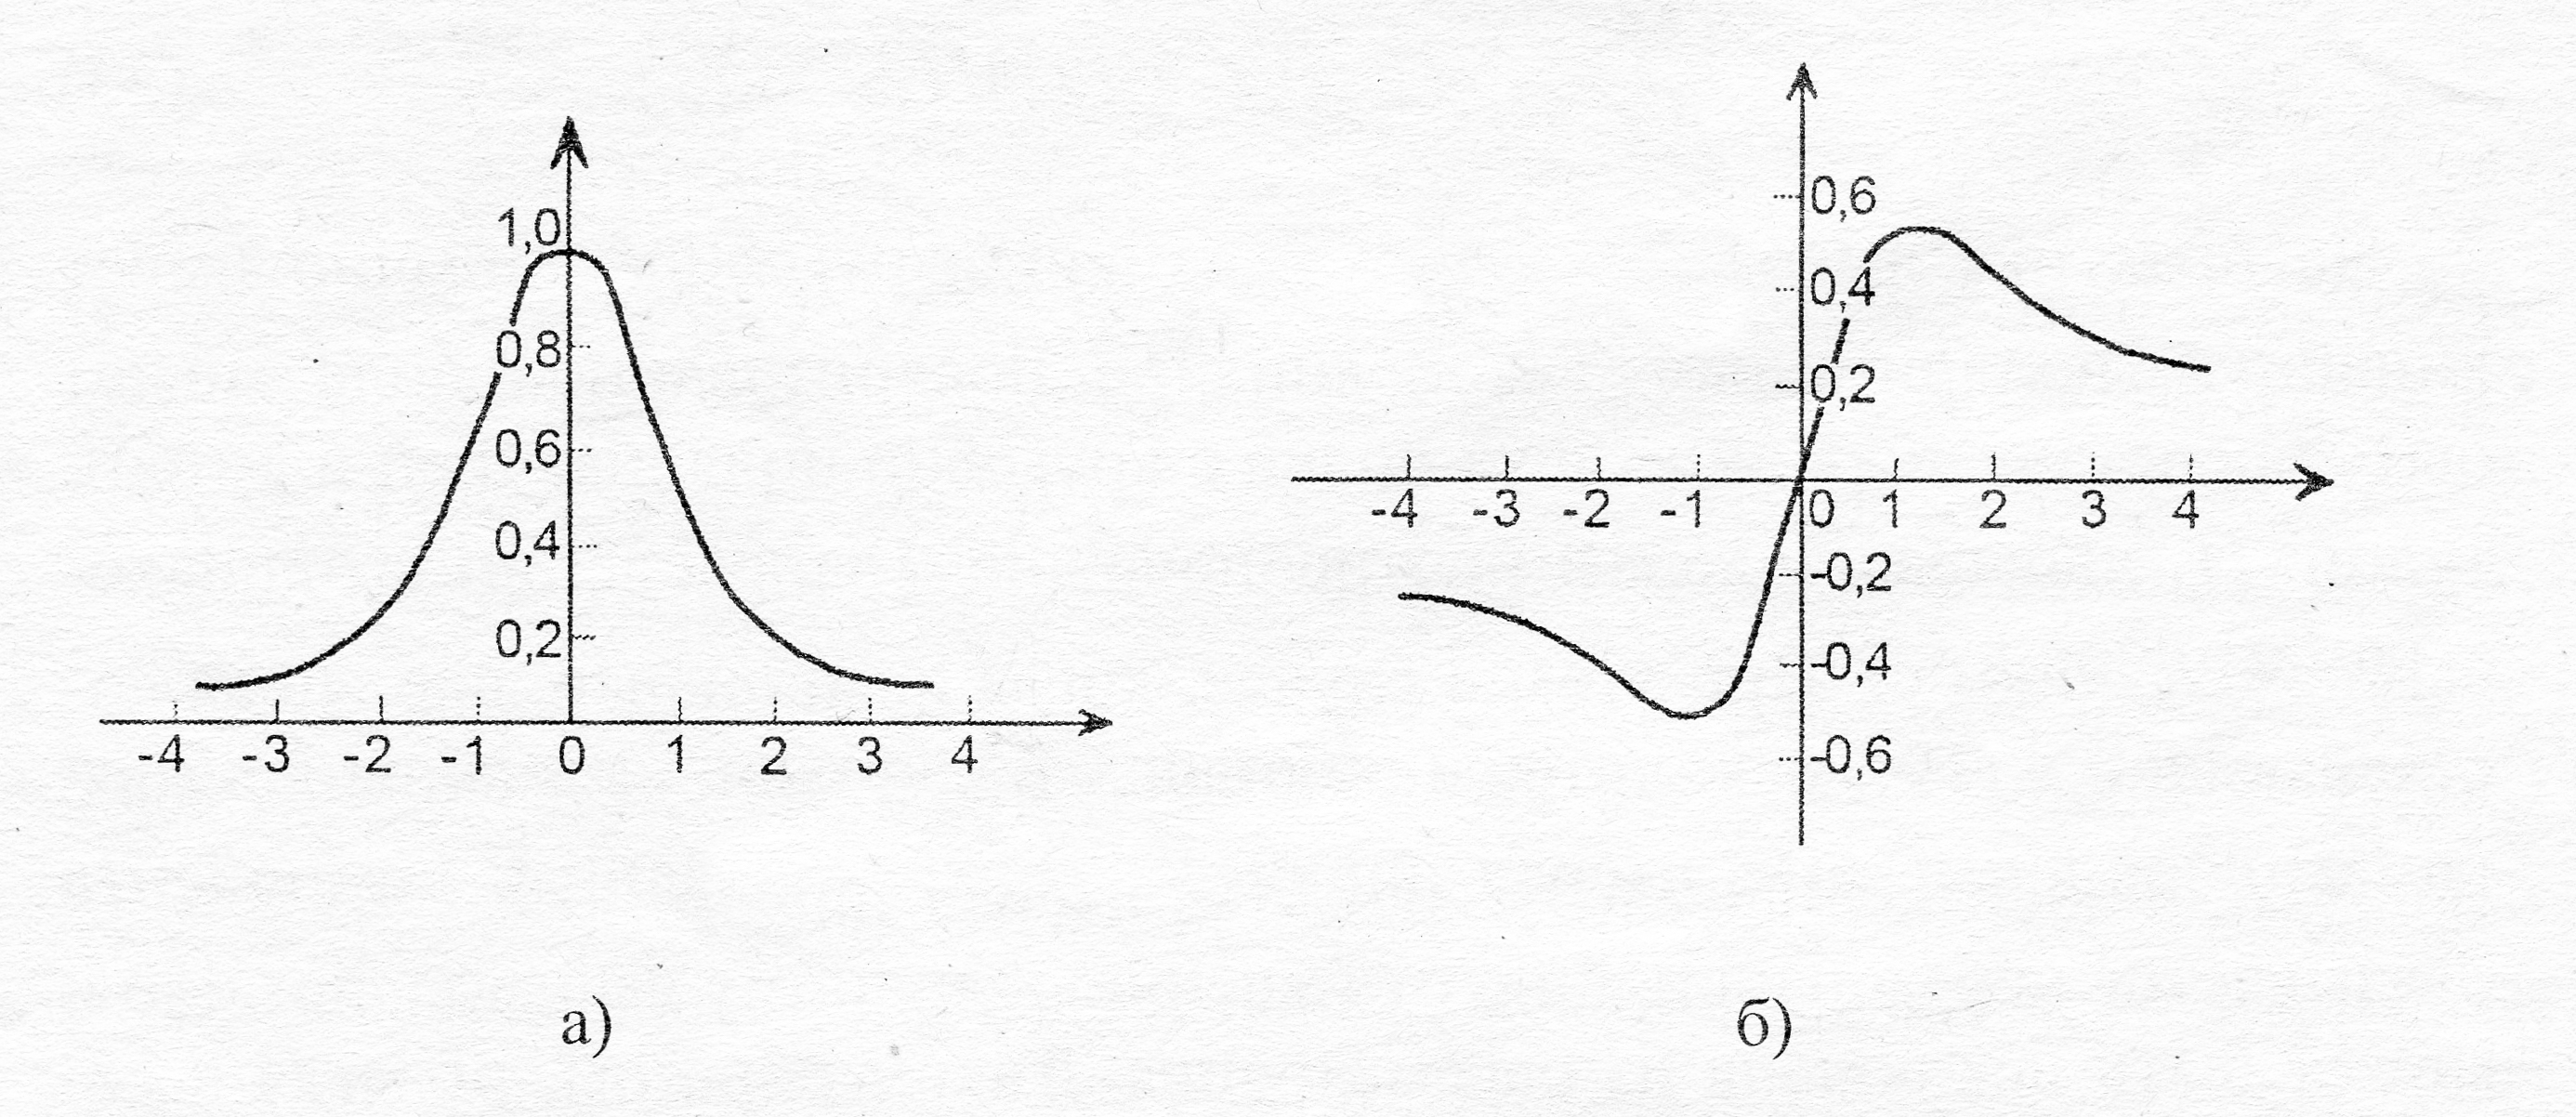
\includegraphics[width=\linewidth]{fig/norm.jpg}
	\caption{Нормированная кривая поглощения (а) и кривая дисперсии (б)}
	\label{fig:5}
\end{figure}

Здесь частота генератора $\nu=8.99$ ГГц. Сигнал появляется при значении тока $I=159 mA$, что соответствует полю в 3550 Гс и исчезает при $I=169 mA$, что соответствует полю 3750 Гс. Пересчет производится по графику зависимости напряженности магнитного поля $H_0$ от тока, протекающего через катушки электромагнита:
\begin{figure}[H]
	\centering
	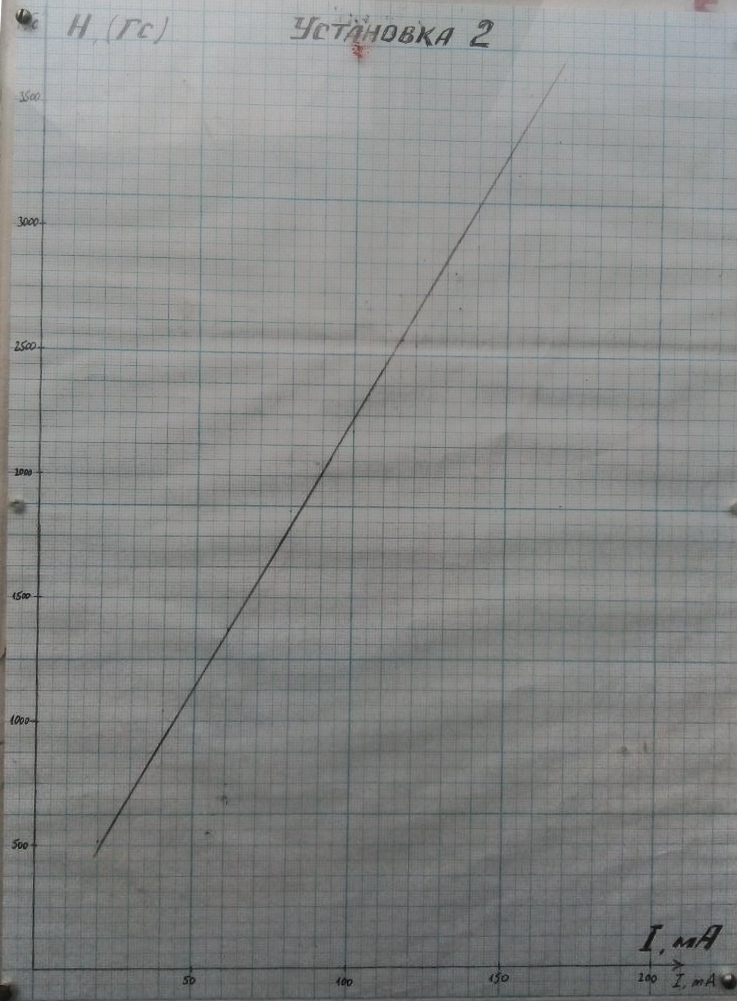
\includegraphics[width=0.9\linewidth]{fig/grad-3.jpg}
	\caption{Градуировочный график}
	\label{fig:6}
\end{figure}

Таким образом, для наблюдаемого сигнала вместо резонансного значения магнитного поля наблюдается целая полоса значений, соответствующая резонансу. 

Далее измерение ширины линии поглощения сигнала ЭПР в единицах поля. 
\begin{gather*}
 	\Delta \omega=\frac{|e|\Delta H_0}{m_e c},
\end{gather*}
где $|e|=4.8 \cdot 10^{-13}$ед, $m=9 \cdot 10^{-31}$ кг, $c=3 \cdot 10^{10}$ см. 
\begin{gather*}
 	\Delta L=3 \text{кл}, \\
 	\Delta I= |160-164| mA, \\
 	\Delta H= 3625-3537.5=87.5 \text{Гс}, \\
 	87.5 / 3 = 29.1, \\
 	\delta H = 0.4 \cdot 29.1 = 11.7 \text{Гс}.
\end{gather*}

Ширина линии поглощения в единицах частоты
\begin{gather*}
 	\Delta \omega_{\text{прак}}=2.08 \cdot 10^{8} c^{-1}, \\
 	\Delta T_{\text{2прак}} = 0.96 \cdot 10^{-8} c, \\
 	\delta H_{\text{теор}}= 2.7 \text{Гс}, \\
 	\Delta \omega_{\text{теор}}= 0.5 \cdot 10^{8} c^{-1}, \\
 	\Delta T_{\text{2теор}} = 4 \cdot 10^{-8} c.
\end{gather*}

Определим число парамагнитных частиц. Для калибровки тракта усиления используется режим модуляции СВЧ-генератора меандром. Такой режим модуляции позволяет получить в схеме возбуждение резонатора переменным СВЧ-сигналом, амплитудный размах которого будет совпадать с реализованным ранее случаем непрерывного возбуждения. Таким образом, регистрация СВЧ-меандра как искусственно вводимого в систему эталонного переменного сигнала позволяет по существу прокалибровать вертикальную ось шкалы осциллографа и позволяет провести сравнение эталонного размаха меандра $L_M$ и наблюдаемого сигнала поглощения $L_C$. У нас: $L_C/L_M=2.3/84=0.027$. По формуле
\begin{gather*}
 	N_0=\frac{3kT}{8\pi Q \mu^2\omega_0 T_2^*}\frac{L_c}{L_M}\frac{P_M}{P_{\text{п}}}\frac{V_\text{рез}}{V_\text{обр}},
\end{gather*}
где $Q=5000, \frac{V_\text{рез}}{V_\text{обр}}=200, \frac{P_M}{P_{\text{п}}}=1, T=300 K, \omega_0=5.64 \cdot 10^{10} c^{-1}, \mu \sim 10^{-6}, T_2^* = 0.96 \cdot 10^{-8} c, k=1.38 \cdot 10^{-16}$ Дж/К. Получаем количество парамагнитных частиц
\begin{gather*}
 	N_0=9.8 \cdot 10^{-9}.
\end{gather*}

\subsection{ЭПР в кристалле рубина}
Измерения проводятся на рубине с активными ионами $Cr^{3+}$. Здесь частота генератора $\nu=8.965$ ГГц. Сигнал появляется в диапазоне значений тока $\Delta I_1=151 - 139 ~mA$, что соответствует полям в 3350 - 3087 Гс и  $\Delta I_2=41 - 34~ mA$, что соответствует полям 925 - 800 Гс. Пересчет производится по графику зависимости напряженности магнитного поля $H_0$ от тока, протекающего через катушки электромагнита. Диапазон $\Delta I_1$ соответствует переходу $-1/2 \rightarrow 1/2$, $\Delta I_2$ - переходу $3/2 \rightarrow 1/2$.

Далее измерение ширины линии поглощения сигнала ЭПР в единицах поля для перехода $-1/2 \rightarrow 1/2$. 
\begin{gather*}
 	\Delta L=2 \text{кл}, \\
 	\Delta I= |48-44| mA, \\
 	\Delta H= |1100-1012.5|=87.5 \text{Гс}, \\
 	75 / 2 = 43.8, \\
 	\delta H = 1 \cdot 43.8 = 43.8 \text{Гс},
\end{gather*}
и время поперечной релаксации
\begin{gather*} 	
	\Delta \omega_{\text{прак}}=7.8 \cdot 10^{8} c^{-1}, \\
 	\Delta T_{\text{2прак}} = 0.26 \cdot 10^{-8} c.
\end{gather*}

Отношение интенсивностей сигналов, соответствующих переходам $-1/2 \rightarrow 1/2$ и $3/2 \rightarrow 1/2$: $1.2/2=0.6$.

Определим число парамагнитных частиц. Здесь У нас: $L_C/L_M=0.003/0.11=0.027$. $Q=5000, \frac{V_\text{рез}}{V_\text{обр}}=200, \frac{P_M}{P_{\text{п}}}=1, T=300 K, \omega_0=5.63 \cdot 10^{10} c^{-1}, \mu \sim 5 \cdot 10^{-7}, T_2^* = 0.26 \cdot 10^{-8} c, k=1.38 \cdot 10^{-16}$ Дж/К. Получаем количество парамагнитных частиц
\begin{gather*}
 	N_0=9.1 \cdot 10^{-9}.
\end{gather*}

\section{Заключение}
В качестве заключения приведем ответ на вопрос 9 - найти теоретическое значение для отношения интенсивностей переходов $-1/2 \rightarrow 1/2$ и $3/2 \rightarrow 1/2$.
\begin{gather*} 	
	E_{3/2} \rightarrow E_{1/2} \\
	\widehat{S_-}\chi_{3/2,1/2} = \hbar \sqrt{\frac32(\frac32+1)-\frac32(\frac32-1)}\chi_{3/2,1/2} = \sqrt{3} \hbar \chi_{3/2,1/2}; \\
	E_{-1/2} \rightarrow E_{1/2} \\
	\widehat{S_+}\chi_{3/2,-1/2} = \hbar \sqrt{\frac32(\frac32+1)+\frac12(-\frac12+1)}\chi_{3/2,1/2} = 2 \hbar \chi_{3/2,1/2}; \\
	\frac{I_{3/2 \rightarrow 1/2}}{I_{-1/2 \rightarrow 1/2}} = \frac{\sqrt{3}}{2}.
\end{gather*}
\end{document}
